\chapter{Implementation details}

We chose for an approach using an intermediate representation.
While an intermediate representation is not strictly necessary for our language, we found that it simplified development.
The intermediate representation allowed us to work on the front end and back end compiler at the same time, without having to discuss many things, which sped up the development process.

The central part of our application, which ties everything together, is the \code{Main} class.

\section{Front end compiler}

The front end compiler is an Antlr 4 listener.
The listener builds a program using objects from the intermediate representation (which is discussed later on).
The front end compiler also checks the program for errors.

In case an error occured, the front end compiler tries to continue.
While this process can yield incorrect errors, which will mainly be caused by an earlier error, it can provide the user more errors in a single pass.
This way he has the ability to fix all errors at once.

\section{Intermediate representation}

The intermediate representation allows us to represent a program as a tree of Java objects.
This helps on the front end side by making the visitor easier as in most cases a visitor method only has to create a new object and add it to the right parent.
Intermediate classes do type checking where possible.

The intermediate representation can be used with other source and target languages.
However, it has been designed for OTLD as source languages, so it might miss some or many features which are necessary to completely support other source languages.

Target languages are supported through the abstract \code{Compiler} class, which provides a structure for visitor-based back end compilers.

Details on the different classes can be found in the Javadoc of the \code{intermediate} package. The class diagram of this package has been included on page \pageref{fig:class_diagram__intermediate}.

\section{Back end compiler}

The back end compiler is an implementation of the \code{Compiler} abstract class of the intermediate representation.
This means that it uses a visitor pattern to go through the tree of intermedate representation objects.
The back end compiler uses an ASM \code{ClassWriter} to create the program.
ASM is described in detail on page \pageref{subj:asm}.
The detailed description for each visitor method can be found in the Javadoc for the \code{jvm} package.

The back end compiler builds a Java class file from scratch.
The program code is put in the static main method, so the class file can be executed directly.
The class (and file) name correspond to the name of the program.
User-defined functions are added as public methods, and user-defined variables as public fields.
The class diagram of the back end compiler has been included on page \pageref{fig:class_diagram__jvm}.

\begin{landscape}
\begin{figure}[p]
\centering
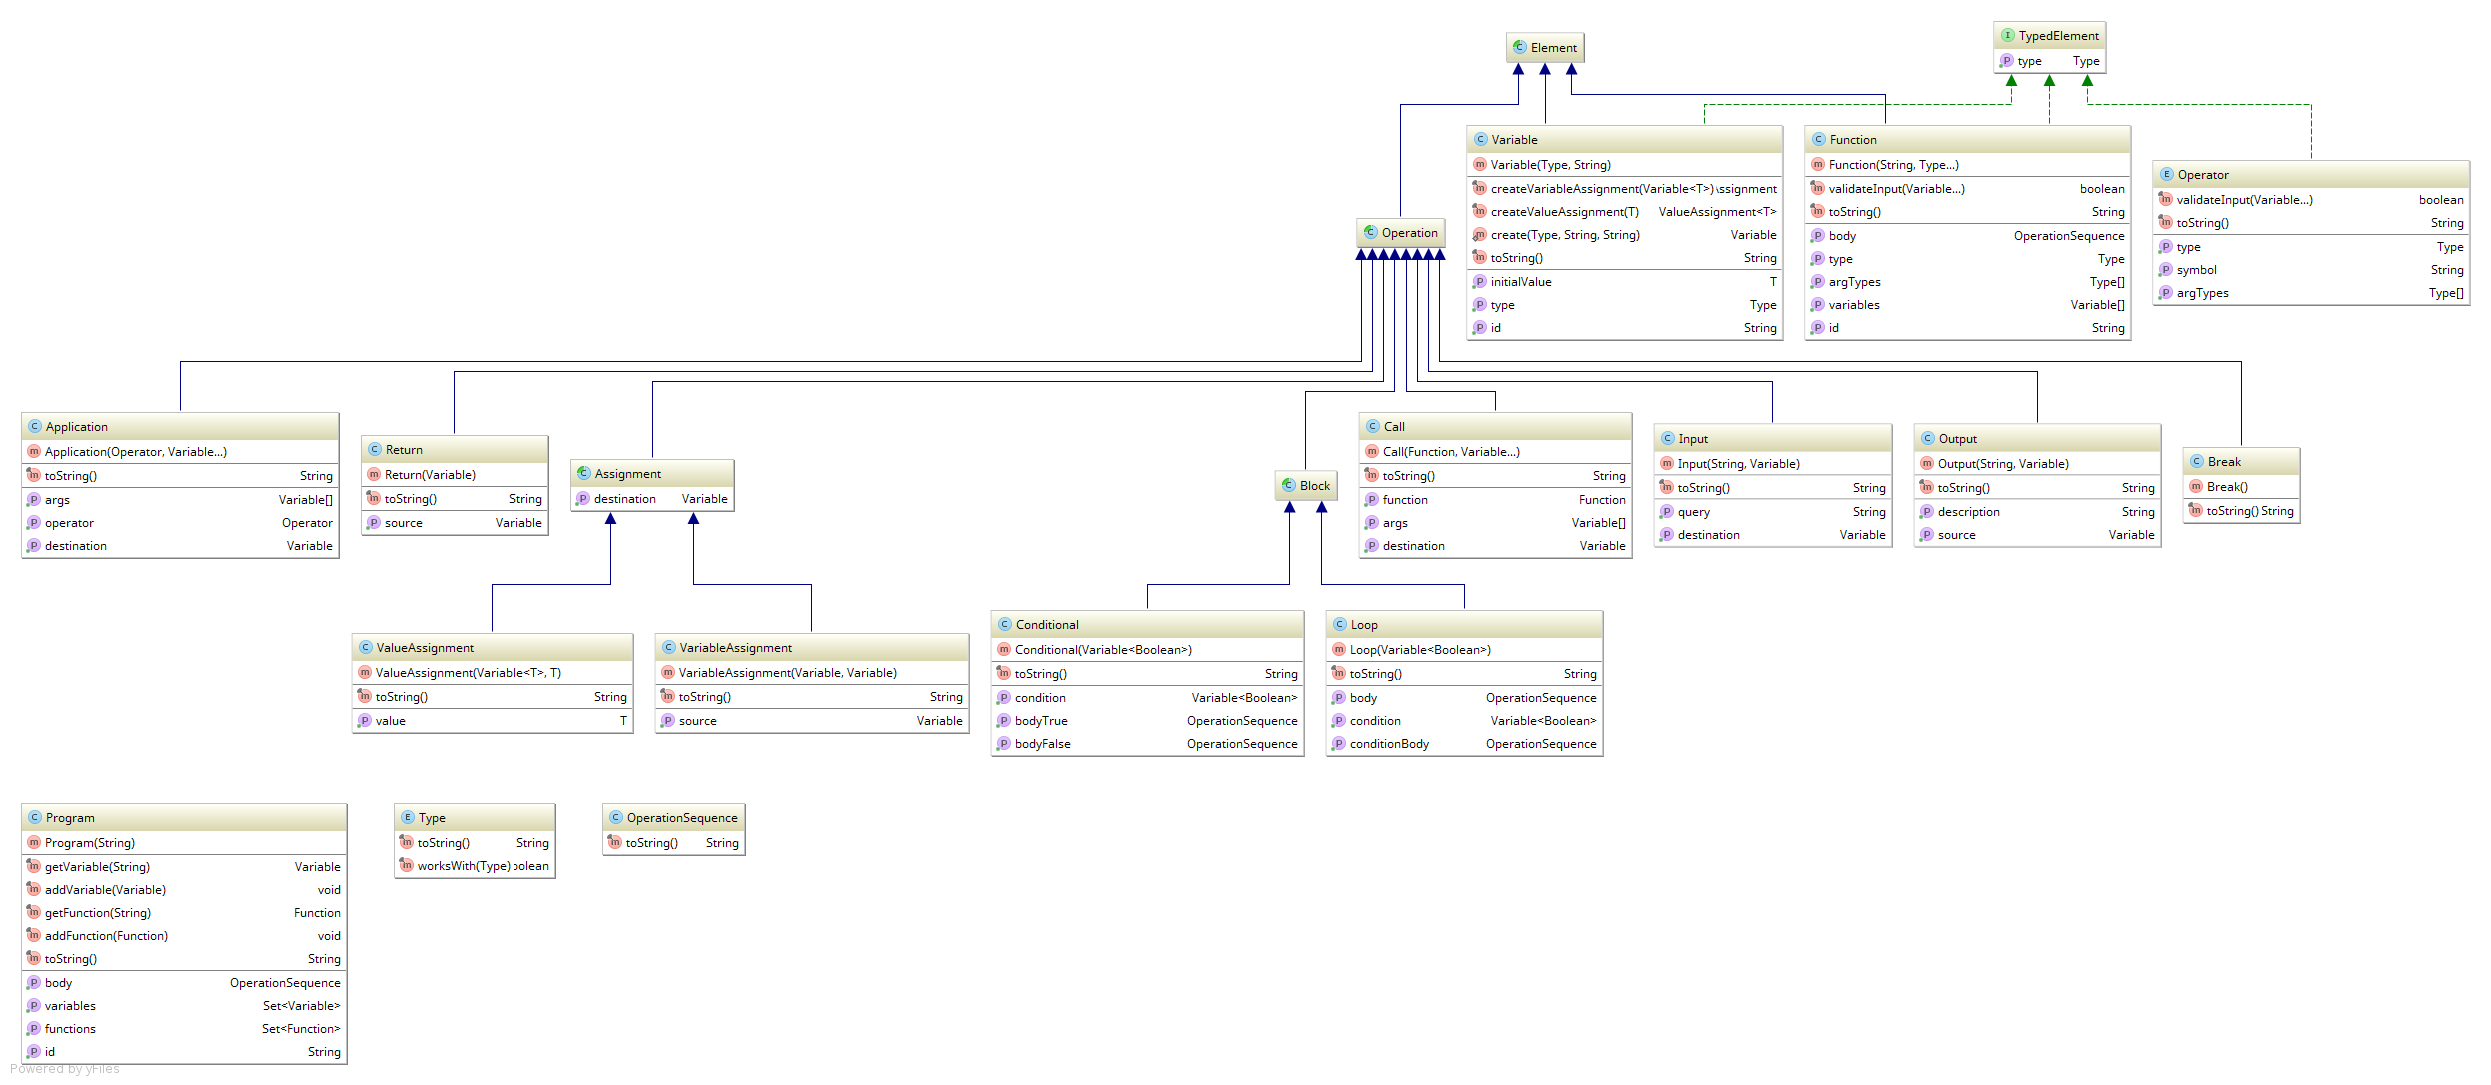
\includegraphics[scale=0.25]{Images/class_diagram__intermediate}
\caption{Class diagram for the intermedate representation}
\label{fig:class_diagram__intermediate}
\end{figure}
\end{landscape}

\begin{figure}[p]
\centering
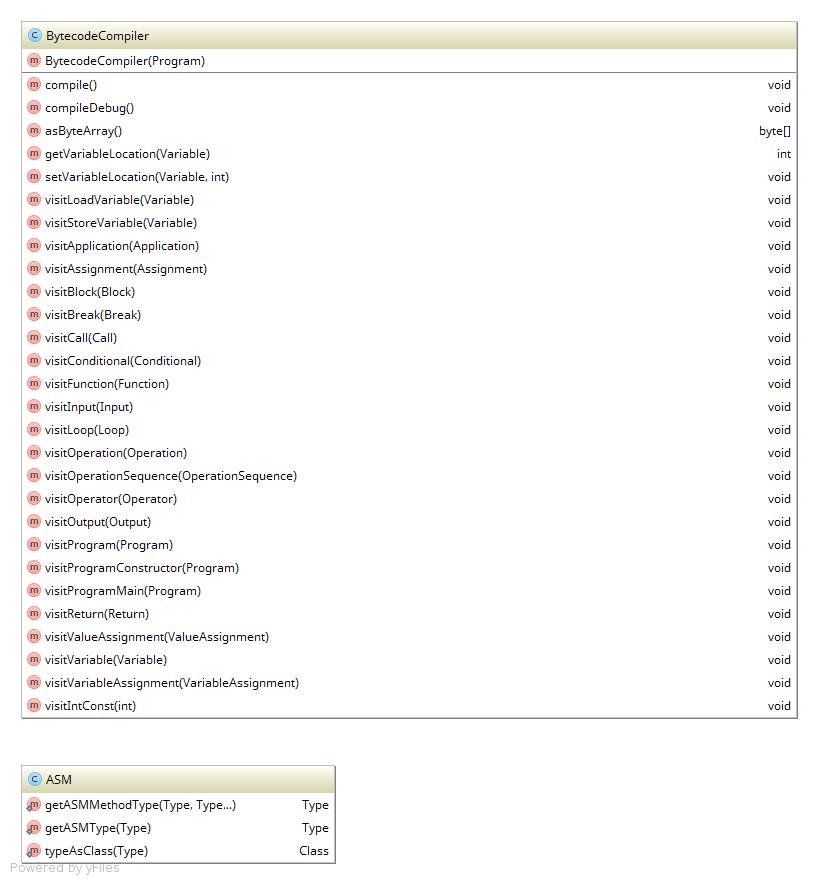
\includegraphics[scale=0.25]{Images/class_diagram__jvm}
\caption{Class diagram for the back end compiler}
\label{fig:class_diagram__jvm}
\end{figure}
